\documentclass[journal]{IEEEtran}
% \documentclass[conference]{IEEEtran}
% \IEEEoverridecommandlockouts
% The preceding line is only needed to identify funding in the first footnote. If that is unneeded, please comment it out.
\usepackage{amsmath,amssymb,amsfonts}
\usepackage{pifont}% http://ctan.org/pkg/pifont
\usepackage{algorithmic}
\usepackage{graphicx}
\usepackage{textcomp}
\usepackage{xcolor}
\usepackage{multirow}
\usepackage{array}
\usepackage[font=small, labelfont=bf]{subfig}
\usepackage[style=ieee, autocite=inline]{biblatex}
\addbibresource{ZoteroLibrary.bib}

\DeclareMathOperator*{\argmin}{\arg\!\min}
\newcommand{\cmark}{\ding{51}}%
\newcommand{\xmark}{\ding{55}}%
\newcolumntype{C}[1]{>{\rule{0pt}{3ex}\centering\arraybackslash}m{#1}} % define new column type


\begin{document}

\title{Discrete-time Control Contraction Metrics (DCCM) for Quasistatic Planar Pushing using Smoothed Dynamics\\
{\footnotesize MIT 2.152[J] Nonlinear Control Project Report}
}

\author{\IEEEauthorblockN{Shao Yuan Chew Chia}
\IEEEauthorblockA{
\textit{Harvard University}\\
Cambridge, MA \\
shaoyuan\_chewchia@college.harvard.edu
}}

\maketitle

\begin{abstract}
The paper explores the feasibility and performance of Discrete-time Control Contraction Metrics (DCCM) on a planar pushing system with smoothed dynamics, to address the challenges of non-smoothness and underactuation of control through contact. While they were unable to achieve many of the theoretical advantages of the control contraction metric framework, they managed to demonstrate the feasibility of synthesizing and running a DCCM controller on a planar pushing system with highly smoothed dynamics. The limitations and gaps in applying their implentation in the real world are also discussed. The paper serves as a good starting point for future work to realize the full potential of DCCMs applied to systems with contact.
\end{abstract}

\section{Introduction} \label{sec:introduction}
% Control through contact is important
Planning and control through contact is an important capability in robotics. In order for robots to manipulate objects in their environment, they need to be able to reason about how to make and break contact. However, this has proved challenging for model-based methods due to two factors:
\begin{enumerate}
	\item{\bf Non-smooth or hybrid nature of contact dynamics}. Contact dynamics involve different modes of contact (e.g. sticking, sliding, no-contact), each with smooth but different dynamics and constraints. When switching between modes, the dynamics are discontinuous and change abruptly. This poses problems for gradient-based methods such as optimal control, as their locally linear models constructed using gradients quickly become inaccurate \autocite{pangGlobalPlanningContactRich2023}.
	\item{\bf Underactuatedness of the system}. Systems that involve contact are underactuated as the state of the unactuated objects cannot be controlled directly. Instead, control inputs to the robot are mediated through friction cones at contact points between the robot and the object, thus severely limiting the control authority of the inputs.
\end{enumerate}

% Current methods for control through contact
Current methods for model based planning and control through contact typically fall into one of three categories: methods that apply smoothing to the dynamics \autocite{stewartOptimalControlSystems2010,pangGlobalPlanningContactRich2023}, methods that explicitly enumerate the contact modes \autocite{hoganFeedbackControlPusherSlider2016}, and methods that implicitly reason about the contact modes \autocite{sleimanContactImplicitTrajectoryOptimization2019,nakatsuruImplicitContactRichManipulation2023,posaDirectMethodTrajectory2014}. Two methods that have been applied to the control of nonlinear underactuated systems are Linear Quadratic Regulator (LQR)-Trees and Control Contraction Metrics (CCMs). LQR-Trees use locally optimal linear control policies to stabilize planned trajectories. Each trajectory has a basin of attraction and these regions are pieced together to cover a larger region of state space.
LQR Trees \autocite{tedrakeLQRtreesFeedbackMotion2010}. Control Contraction Metrics, first established in \autocite{manchesterControlContractionMetrics2017}, were shown to be effective at controling underactuated systems in \autocite{manchesterUnifyingRobotTrajectory2018}.

% Why we would want to use Control Contraction Metrics
Control Contraction Metrics (CCM)s theoretically provide 4 key advantages over other control methods as described in \autocite{manchesterControlContractionMetrics2017,manchesterUnifyingRobotTrajectory2018,singhRobustOnlineMotion2017,weiControlContractionMetric2021}:
\begin{enumerate}
	\item {\bf Certificates of stability and convergence rates}. In general, nonlinear MPC does not provide guarantees on stability or performance. While Control Lyapunov Functions (CLFs) and LQR based methods can produce certificates, the guarantees provided by CCMs are not tied to specific equilbria or trajectories.
	\item {\bf Trajectory independent controllers}. CCMs generate controllers that stabilize every feasible trajectory in a region, while CLFs and LQR based methods require designing controllers for each trajectory and stitching them together to cover larger regions.
	\item {\bf Convex synthesis of the controller}. The control synthesis problem can be formulated as a convex optimization problem, which is easier to solve numerically and can leverage powerful tools like SOS programming.
	\item {\bf Faster online computation of the control law}. The online computation of the geodesic in CCMs is typically simpler than the nonlinear MPC optimal control problem.
\end{enumerate}

% What are we doing in this paper
In this paper we use the analytic smoothing of contact dynamics described in \autocite{pangGlobalPlanningContactRich2023} to address the challenge of non-smoothness, and explore the effectiveness of building a Discrete-time Control Contraction Metric (DCCM) as demonstrated by \autocite{weiControlContractionMetric2021} on top of that smoothed system to handle the underactuatedness and nonlinearity of the system. Our hope was that we would be able to synthesize a DCCM for a system with low amounts of smoothing and that this controller would also stabilize a "real-world" system with exact dynamics, however we did not manage to achieve that goal. We only managed to synthesize a controller that worked around a particular desired trajectory under significant smoothing, but are hopeful that our findings in this paper will serve as a good jumping off points for future work to realize the full potential of DCCMs applied to systems with contact.

\section{Preliminaries and Problem Formulation}
\subsection{Quasistatic Assumptions}
We will assume that our system is quasistatic, meaning at each time step velocities and accelerations of the system are 0. This corresponds to having a high amount of damping and is a reasonable assumption in the 2D planar pushing setup where we restrict pushing velocities to be low and there is a large amount of friction between the object and table surface. As a result, the state of our system only consists of positions.

\subsection{Analytically Smoothed Contact Dynamics}
In this work we use the analytically smoothed contact dynamics and corresponding simulator developed by \autocite{pangGlobalPlanningContactRich2023}. Contact dynamics are formulated as an unconstrained convex program where the contact and friction contraints are moved into the objective function using a log barrier function. The effect of this is that there is a log barrier penalty for violating the contact constraints. Constraints can exert force even if they are not active and this translates to producing a force at a distance.

We plot the force at a distance effect of the smoothed contact dynamics in Figure \ref{fig:smoothed_contact_dynamics}. We see that for a high weight, which corresponds to a small force at a distance, the next $b_x$ is close to 0, but as the log barrier weight decreases, the box is pushed further to the right.

% Figure showing force at a distance
\begin{figure}[t]
	\centering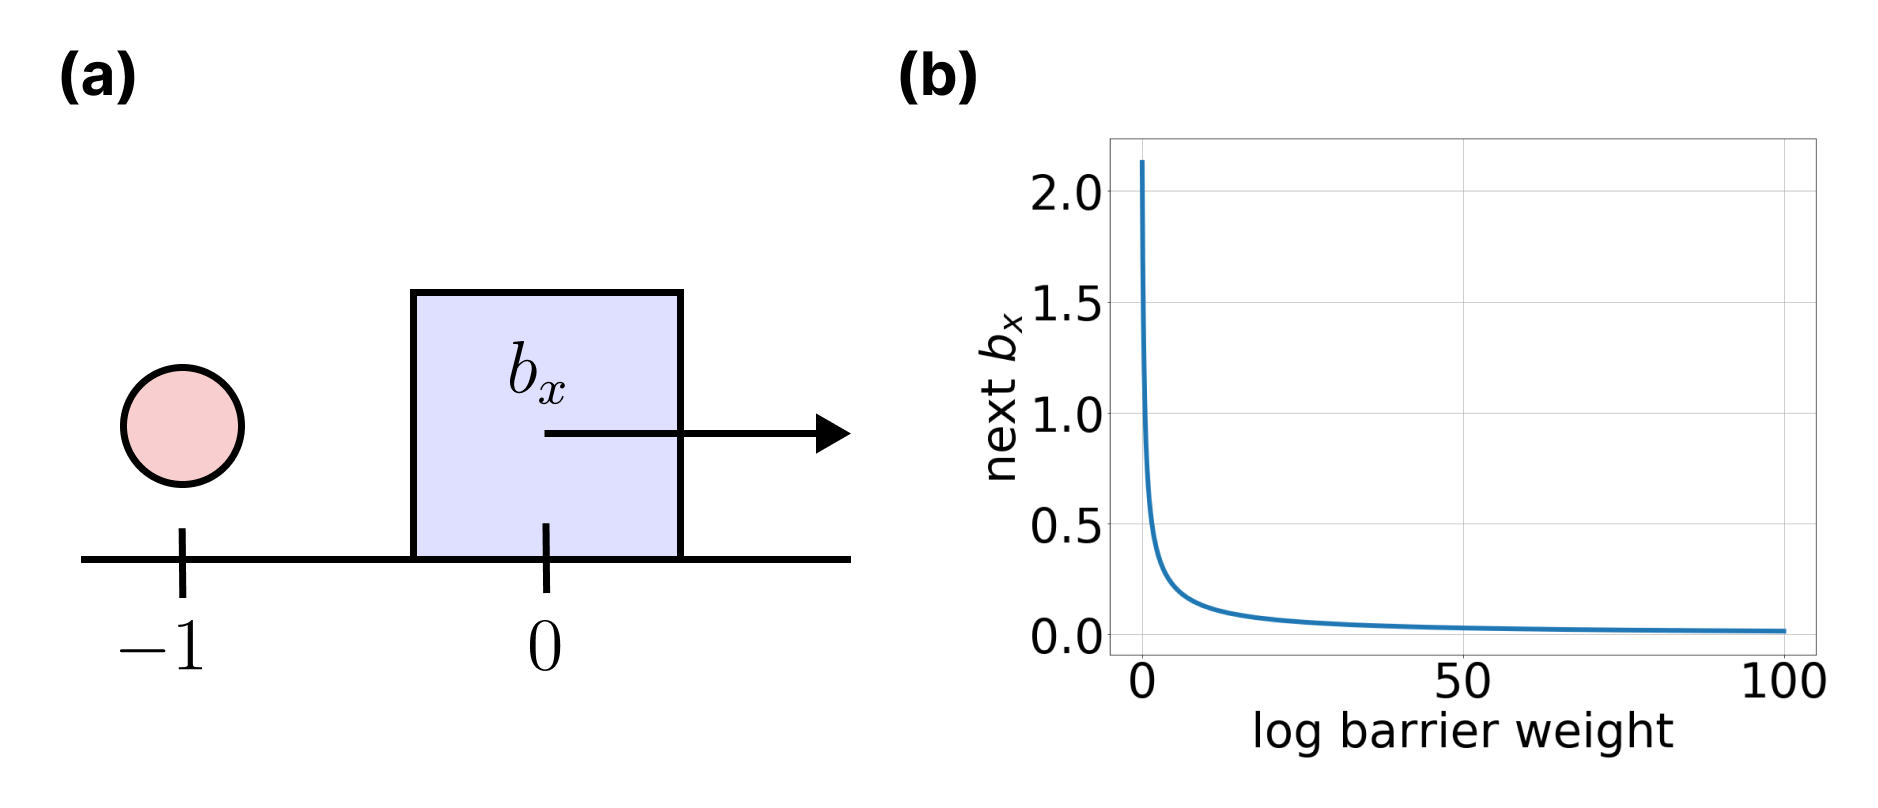
\includegraphics[width = 0.45 \textwidth]
	{figures/smoothed_contact_dynamics.png}
    \caption{Force at a distance effect of smoothed contact dynamics. (\textbf{a}) A system consisting of an actuated point finger at $x=-1$ and unactuated box at $x=0$. (\textbf{b}) The next $b_x$ after rolling out one step of the analytically smoothed dynamics with different log barrier weights.}
	\label{fig:smoothed_contact_dynamics}
	\vskip -0.25 true in
\end{figure}

\subsection{Planar Pushing System}
The state of 
\begin{equation}
    x = \begin{bmatrix}b_x & b_y & b_{\theta}& s_x& s_y\end{bmatrix}^\top
\end{equation}

control input $u$ are absolute position commands for the sphere
\begin{equation}
    u = \begin{bmatrix}u_x\\ u_y \end{bmatrix}
\end{equation}

The system evolves in nonlinearly in discrete time and is control affine. The dynamics are defined as

\begin{equation}
    x_{k+1} = f(x_k) + g(x_k)u_k
\end{equation}

where $f$ and $g$ are smooth functions due to the smoothing of the contact dynamics described in the previous section.

The differential dynamics are defined as
\begin{equation}
    \delta_{x_k} = A(x_k)\delta_{x_k} + B(x_k)\delta_{u_k}
\end{equation}
where $A(x_k) = \frac{\partial (f(x_k) + g(x_k)u_k)}{\partial x_k} \in \mathbb{R}^{5 \times 5}$ and $B(x_k) = \frac{\partial (f(x_k) + g(x_k)u_k)}{\partial u_k} \in \mathbb{R}^{5 \times 2}$ are the Jacobians of the dynamics.

We can define the state feedback control law
\begin{equation}
	\label{eq:delta_control_law}
    \delta_{u_k} = K(x_k)\delta_{x_k}
\end{equation}
where $K$ is the state dependent feedback gain matrix.

Generalized infinitesimal squared distance in the positive definite metric $M$ is denoted $V_k$
\begin{equation}
    V_k = \delta^\top_{x_k} M_{k} \delta_{x_k}
\end{equation}

And by substituting the differential dynamics and control law, we can see that the generalized infinitesimal squared distance at the next time step is

\begin{equation}
	\begin{aligned}
	V_{k+1} & = \delta^\top_{x_{k+1}} M_{k+1} \delta_{x_{k+1}} \\
	& = \delta^\top_{x_k} (A_k + B_k K_k)^\top M_{k+1} (A_k + B_k K_k)\delta_{x_k}
	\end{aligned}
\end{equation}

The contraction condition can then be expressed as
\begin{equation}
	V_{k+1} - V_k \leq 
	- \beta V_k <
	0
\end{equation}

which simplifies to
\begin{equation}
	\label{eq:contraction_condition}
	(A_k + B_k K_k)^\top M_{k+1} (A_k + B_k K_k) - (1 - \beta) M_k < 0
\end{equation}

\autocite{weiControlContractionMetric2021} showed that equation \ref{eq:contraction_condition} can be transformed via Schur's complement (among other transformations) into
% Create a 2x2 matrix
\begin{equation}
	\label{eq:contraction_condition_schur}
	\begin{bmatrix}
		W_{k+1} & A_k + B_k L_k \\
		(A_k + B_k L_k)^\top & (1 - \beta) W_k
	\end{bmatrix} > 0
\end{equation}
where $W := M^{-1}$ and $L := KW$

\section{Methods}
\subsection{Contraction Metric and Controller Synthesis}
\subsubsection{Sum of Squares (SOS) Programming}
In order to synthesize the contraction metric and controller, we use the SOS programming framework described in \autocite{weiControlContractionMetric2021} with some slight modifications.

\begin{equation}
	\label{eq:dccm_opt}
	\begin{aligned}
	\min_{l_c, w_c, r} & r \\
	s.t. & \forall k, w^\top \Omega w - r w^\top w \in \Sigma(x_k, u_k, w) \\
	& r \geq 0.1
	\end{aligned}
\end{equation}

where $\Sigma(x_k, u_k, w)$ is the set of SOS polynomials that satisfy the contraction condition in equation \ref{eq:contraction_condition_schur}. $l_c$ are the polynomial coefficients of $L$ and $w_c$ are the polynomial coefficients of $W$.
\begin{equation}
	\label{eq:dccm_opt_params}
	\begin{aligned}
	\Omega &=
	\begin{bmatrix}
		W_{k+1} & A_k + B_k L_k \\
		(A_k + B_k L_k)^\top & (1 - \beta) W_k
	\end{bmatrix} \\
	% W_k is a 5x5 symmetric matrix
	W_k &= 
	\begin{bmatrix}
		W_{11_k} & W_{12_k} & W_{13_k} & W_{14_k} & W_{15_k} \\
		W_{12_k} & W_{22_k} & W_{23_k} & W_{24_k} & W_{25_k} \\
		W_{13_k} & W_{23_k} & W_{33_k} & W_{34_k} & W_{35_k} \\
		W_{14_k} & W_{24_k} & W_{34_k} & W_{44_k} & W_{45_k} \\
		W_{15_k} & W_{25_k} & W_{35_k} & W_{45_k} & W_{55_k} \\
	\end{bmatrix} \\
	% L_k is a 2x5 matrix
	L_k &=
	\begin{bmatrix}
		L_{11_k} & L_{12_k} & L_{13_k} & L_{14_k} & L_{15_k} \\
		L_{21_k} & L_{22_k} & L_{23_k} & L_{24_k} & L_{25_k} \\
	\end{bmatrix} \\
	\end{aligned}
\end{equation}

each $W.._{k} = w.._c v(x_k)$ is a polynomial constructed from the row vector of coefficients of $w.._c$ and the monomial basis vector $v(x_k)$. For example, if the degree of the polynomial is chosen to be $4$,
\begin{equation}
	v(x_k) = [x^4_{k_4}, x_{k_3}x^3_{k_4}, x^2_{k_3}x^2_{k_4}, \cdots ,x_{k_1}, x_{k_0}, 1]
\end{equation}
where $v(x_k)$ has $126$ elements. $L.._k = l.._c v(x_k)$ is similarly defined.

In general, the dimensions of the matrices are as follows: $\Omega: 2 \cdot dim(x) \times 2 \cdot dim(x), W: dim(x) \times dim(x), L: dim(u) \times dim(x)$

We note the difference in the way we use the slack variable $r$ compared to \autocite{weiControlContractionMetric2021}. In \autocite{weiControlContractionMetric2021}, the constraints on the optimization program are $w^\top \Omega w - r I \in \Sigma(x_k, u_k, w), r \geq 0$. In practice we found that in some cases, especially when generating a higher degree metric, that the solver would return a trivial solution where $r$, $w_c$ and $l_c$ are extremely small numbers (on the order of $1e-17$). By setting a higher bound on $r$, we force the solver to find a solution where the contraction condition is satisfied with a greater buffer and the returned coefficients of $w_c$ and $l_c$ are larger.

Another difference is that we do not have closed form equations for the $A$ and $B$ matrices which would allow us to enforce the contraction conditions over all states. Instead, we sample a set of state, control action pairs and enforce the contraction condition over these samples. We use the contact dynamics solver described in \autocite{pangGlobalPlanningContactRich2023} to calculate the next state $x_{k+1}$, and the Jacobians $A_k$ and $B_k$, for each sample of the current state $x_k$ and control action $u_k$, and substitute these values into the constraints in optimization program (\ref{eq:dccm_opt}). Since $M$ is smooth, we can expect the contraction condition to be satisfied over at least a small local region around each sample. However, if the samples are too sparse, the contraction condition may not be satisfied over all the states around the desired trajectory.

We solve this SOS program using Drake's Mathematical Program \autocite{DrakeModelBasedDesign}, which uses Mosek under the hood to solve this Semidefinite Program (SDP).

\subsubsection{Sampling Strategy}
To get a contraction metric valid over the entire state space we would have to densely sample the entire state space. However, the available RAM on the machine sets an upper bound of the size of the optmization program, which for a monomial basis of degree $4$, was around $2000$ samples. Thus, to get a contraction metric and controller that had good performance at least in the vicinity of the desired trajectory, we only sampled states and control actions from a small region around the desired trajectory. This is a clear limitation of the current approach and future work would involve finding a way to enforce the contraction condition over a larger portion of state space.

\subsection{Online Geodesic and Controller Computation}
With the contraction metric synthesized, we now need to compute the control action that enforces the contraction condition.

For a smooth curve $c(s), s\in [0, 1]$ that connects two points in state space $x_0$ and $x_1$, \autocite{manchesterControlContractionMetrics2017} defines the Riemannian length and energy of the curve as

\begin{equation}
	\begin{aligned}
		L(c) &= \int_0^1 \sqrt{\frac{\partial{c(s)}}{\partial{s}} ^\top M(c(s)) \frac{\partial{c(s)}}{\partial{s}}} ds \\
		E(c) &= \int_0^1 L(c)^2 ds
	\end{aligned}
	\label{eq:geodesic_length_energy}
\end{equation}

The geodesic $\gamma(x_0, x_1)$ is the curve that minimizes the Riemanian length and energy between $x_0$ and $x_1$

\begin{equation}
	\label{eq:geodesic}
	\begin{aligned}
		\gamma(x_0, x_1) &= \argmin_{c} L(c) \\
		&= \arg \min_{c} E(c)
	\end{aligned}
\end{equation}

By the contraction condition we enforced, we see that the Riemanian energy of geodesic decreases exponentially as the system evolves and thus can be thought of as an incremental Lyapunov function \autocite{manchesterControlContractionMetrics2017}. In order to numerically approximate the geodesic $\gamma(x^*_k, x_k)$, we discretize the curve into $N$ segments and solve the following optimization program

\begin{equation}
	\label{eq:geodesic_opt}
	\begin{aligned}
		\bar{\gamma}(x^*_k, x_k) = \argmin_{ \substack{ x[\cdot], \Delta x_{s}[\cdot],\\ \Delta s[\cdot], m[\cdot], y[\cdot]}}
		& \sum_{i=0}^{N-1} y[i] + \Delta s[i]^2 \\
		s.t. & \forall i, y \geq \Delta s[i] \Delta x_s[i]^\top M(m[i]) \Delta x_s[i]\\
		& x[0] = x^*_k, \quad x[N] = x_k \\
		& \forall i, x[i+1] = x[i] + \Delta x_{s}[i]\Delta s[i] \\
		& \forall i, \Delta s[i] > 0, \quad \sum_{i=0}^{N-1} \Delta s[i] = 1\\
		& \forall i, M(m[i]) W(x[i]) = I  \\
	\end{aligned}
\end{equation}
where $x[i]$ is the state at the start of the $i$th segment of the geodesic, $\Delta s[i]$ is a small positive scalar, $\Delta x_s[i]$ is the discretized displacement vector, $y[i]$ is a slack variable that represents the Riemanian energy and $N$ is the number of segments the $\gamma$ is discretized into. $m[i]$ is a slack variable introduced such that the $5\times5$ symbolic matrix $W(x[i])$ does not need to be explicitly inverted which was found to be a severe computational bottleneck. The constraint $M(m[i]) W(x[i]) = I$ is a surrogate for enforcing $M(m[i])=W(x[i])^{-1}$. Adding $\Delta s[i]^2$ to the objective serves to spread out the discretized points evenly along the geodesic.

As this is a non-convex program, we use Drake, this time using SNOPT under the hood \autocite{DrakeModelBasedDesign}.

With the geodesic $\bar{\gamma}(x^*_k, x_k)$ computed, we can compute the control action $u_k$ that enforces the contraction condition

\begin{equation}
	\label{eq:control_law}
	\begin{aligned}
		u_k &= u^*_k + \sum_{i=0}^{N-1} \Delta s[i] K(x[i]) \Delta x_s[i]  \\
		&= u^*_k + \sum_{i=0}^{N-1} \Delta s[i] L(x[i]) W(x[i])^{-1} \Delta x_s[i]
	\end{aligned}
\end{equation}

An important point to note is that the integration is done from $x^*_k$ to $x_k$ and not the other way around. While it might seem intuitive that we want to calculate the $\delta_u$ that brings the system from $x_k$ to $x^*_k$, this is actually not the right way to think about it. First, the $\delta_u$ in equation \ref{eq:delta_control_law} does not lead to a change in state $\delta_x$ on the right side of the same equation. Instead, \ref{eq:delta_control_law} tells us for a change in state $\delta_x$ from a nominal trajectory, what is the corresponding $\delta_u$ that enforces the contraction condition. In this case, the nominal trajectory is $x^*$ and $u^*$, thus to calculate the $\delta_u$ that enforces the contraction condition, we need to integrate from $x^*_k$ to $x_k$.

\section{Experimental Setup}
\subsection{Creating Feasible Desired Trajectories}
To create the desired trajectory, we first parameterised an arbitrary circular trajectory with the robot "behind" the object at each time step and the object slowly rotating as it travelled around the circle. We then rolled out the dynamics from the initial condition, using the position of the robot at the next time step as the open loop position command for the robot and recorded the actual positions of the object under this open loop control. We created two feasible circular trajectories of slightly different radius in this way and spliced them together in the middle in order to introduce a step change in the desired trajectory. Finally, we introduce an additional initial disturbance by adding an offset to the initial state from the first state of the desired trajectory. We do this process twice to create desired trajectories for both the log barrier weight 10 and 100 levels of smoothing.

\section{Results and Discussion}
Our original goal was to synthesize a DCCM with a small amount of smoothing that would transfer well to stabilizing the real system to arbitrary feasible desired trajectories under non-smooth, exact contact dynamics. Unfortunately, we were not able to achieve this goal. We find that when using a small amount of smoothing, a higher degree monomial basis was required to enforce the contraction condition across all samples. Furthermore, since the dynamics were less smooth, a greater density of samples was required in order for the contraction condition to hold around the desired trajectory. This can be seen from the result in table (\ref{table:results_overview}) where even though we were able to synthesize DCCMs for 500 samples for both log barrier weights, the DCCM for log barrier weight 10 worked while the DCCM for log barrier weight 100 did not.

Both of these factors (requiring a higher degree, and more samples) led to the optimization (\ref{eq:dccm_opt}) being intractable due to the computer used running out of RAM. Ultimately we were only able to find a stabilizing controller for a log barrier weight of 10, which corresponds to the robot exerting $0.1$N of force on an object that is $1$m away.

\begin{table}[h]
	\centering
	\begin{tabular}{| C{0.8cm} | c | c || c | c | c | c | c |} 
		\hline
		Log Barrier Weight  & Deg. & \# Samples 
		& 100 &500 & 1000 & 2000 & 3000\\ \hline\hline
		\multirow{4}{*}{10} & \multirow{2}{*}{4} 
		& Synthesizes 
		& \cmark & \cmark & \cmark & \cmark & ! \\ \cline{3-8}
		& & Stabilzes 
		& \xmark & \cmark & \cmark & \cmark & - \\ \cline{2-8}
		& \multirow{2}{*}{6}
		& Synthesizes 
		& \cmark & \cmark & ! & - & - \\ \cline{3-8}
		& &  Stabilizes
		& \xmark & \xmark & - & - & - \\ \hline
		\multirow{4}{*}{100} & \multirow{2}{*}{4} 
		& Synthesizes
		& \cmark & \cmark & \xmark & - & - \\ \cline{3-8}
		& & Stabilzes
		& \xmark & \xmark & - & - & -\\ \cline{2-8}
		& \multirow{2}{*}{6} 
		& Synthesizes
		& \cmark & \cmark & ! & - & -\\ \cline{3-8}
		& &  Stabilizes
		& \xmark & \xmark & - & - & -\\ \hline
	\end{tabular}
	\caption{Feasibility (whether a DCCM can be synthesized) and performance (whether the found DCCM stabilizes to the desired trajectory) across different log barrier weights (10 is high smoothing, 100 is low smoothing), degree of monomial basis used, and number of sampled points at which the contraction condition is enforced.  Symbols: \cmark (succeeds), \xmark (fails), ! (program crashes), - (did not/could not run test).}
	\label{table:results_overview}
\end{table}

\subsection{Controller Performance}
Figure (\ref{fig:result_2000}) demonstrates the performance of the controller synthesized and run with parameters listed in table (\ref{table:best_params}). We see that the controller is able to stabilize the system from the initial offset at $t=0$ and step change in desired trajectory at $t=5$, with the geodesic energy $E(\bar{\gamma})$ decreasing exponentially after each instantaneous reference change.

\begin{table}[h]
	\centering
	\begin{tabular}{| C{1.5cm} | c | c | c | c |} 
		\hline
		Log Barrier Weight  & Deg. & \# Samples 
		& \# Geodesic Segments & $\beta$ \\ \hline\hline
		10 & 4 & 2000 & 1 & 0.1\\ \hline
	\end{tabular}
	\caption{Parameters of the controller shown in figure (\ref{fig:result_2000}), where \# Geodesic Segments is the parameter $N$ in optimization problem \ref{eq:geodesic_opt}, and $\beta = (1 - \text{convergence rate w.r.t. DCCM})$ as shown in \ref{eq:dccm_opt_params}.}
	\label{table:best_params}
\end{table}

\begin{figure}[h]
	\centering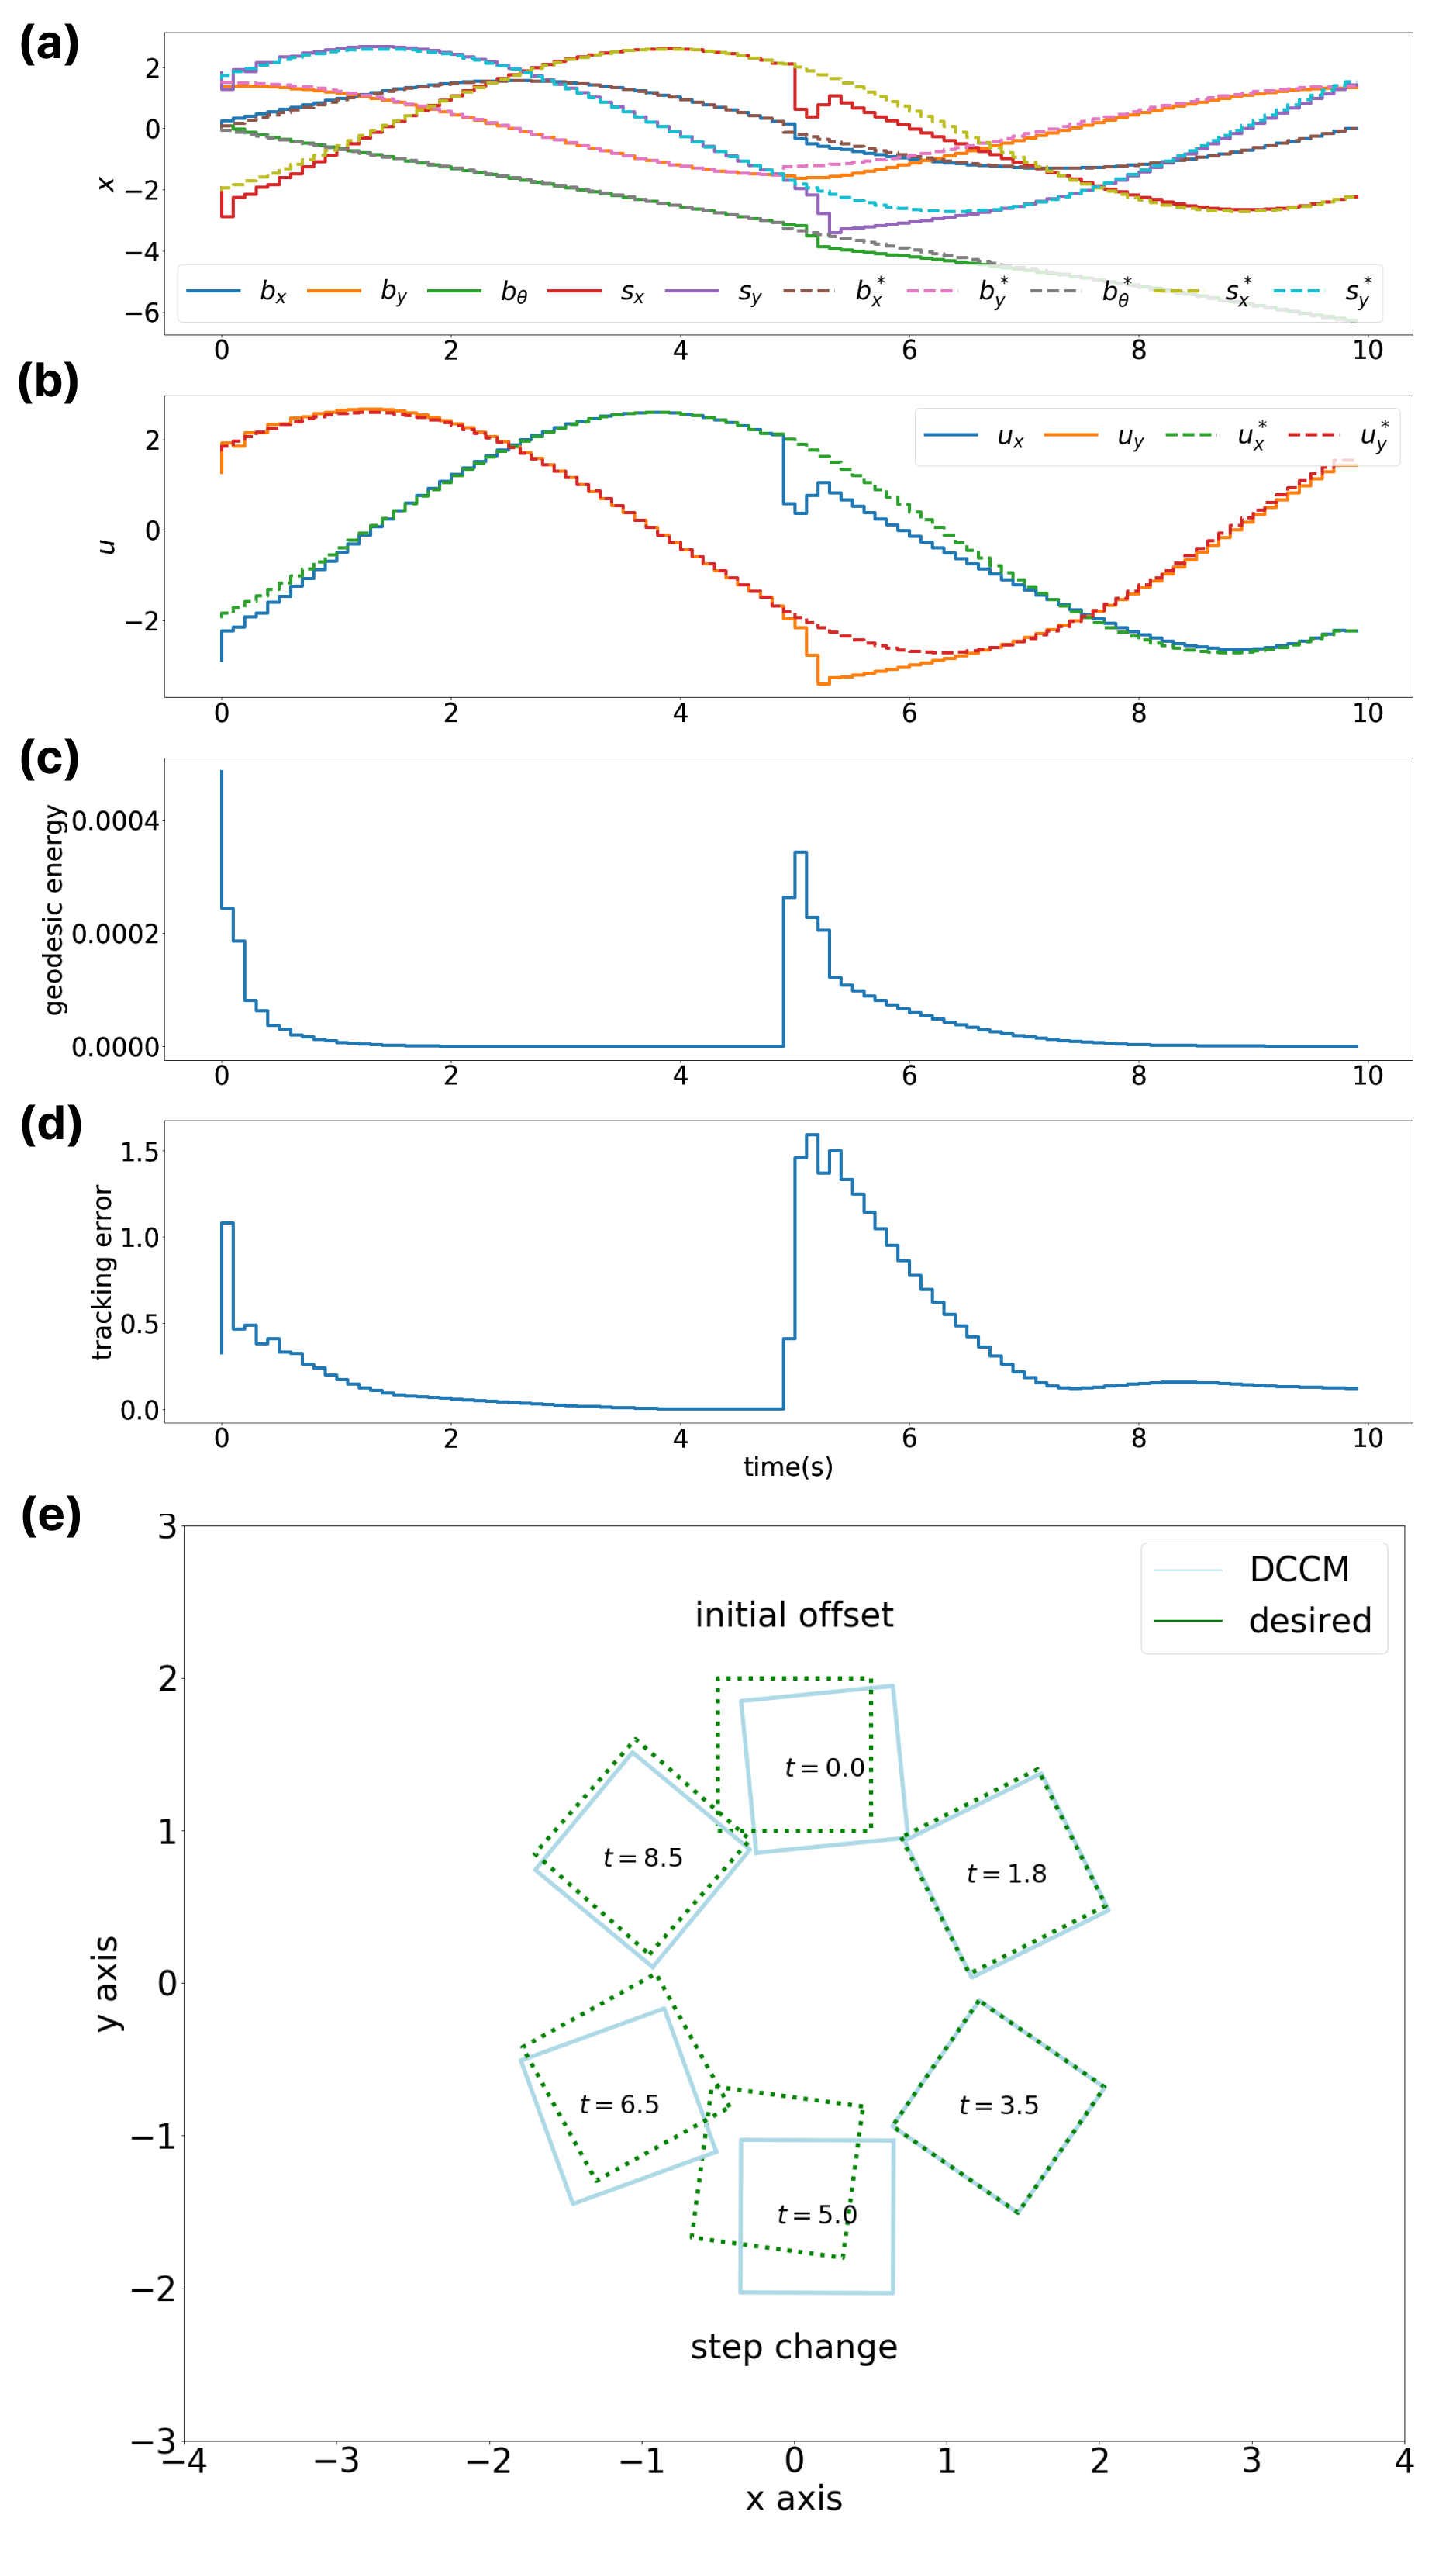
\includegraphics[width = 0.47 \textwidth]
	{figures/result_lbw10_2000samples.png}
    \caption{Performance of DCCM with parameters (\ref{table:best_params}); (\textbf{a}) desired state $x^*$ and actual state $x$; (\textbf{b}) nominal input $u^*$ and DCCM input $u$; (\textbf{c}) geodesic energy $E(\bar{\gamma})$, (\ref{eq:geodesic_length_energy}), (\ref{eq:geodesic_opt}); (\textbf{d}) $l_2$-norm tracking error; (\textbf{c}) desired and actual positions of the box at various time steps.}
	\label{fig:result_2000}
\end{figure}

\subsection{Effect of number of samples on controller performance}
Figure \ref{fig:comparison_num_sample} shows the performance of 3 controllers, synthesized with 500, 1000, and 2000 samples respectively. Note that the controller synthesized with 100 samples was not included in the figure as the controller was not able to stabilize the system. We can see that as the number of samples increases, the controller is better able to regulate the geodesic energy. For the controller with 500 samples, geodesic energy does not exponentially decrease, in fact, it increases at times. We reason that this is due to the contraction condition not being enforced over the states of the trajectory due to the sparse sampling.

It is also interesting to note that even though the 2000 sample controller consistently has the lowest geodesic energy, and fastest decrease in geodesic energy after instantaneous reference change, it also has the largest l2-norm tracking error. In order to stabilize the system and make the geodesic energy decrease exponentialy, the sphere robot has to deviate a greater amount from the reference trajectory in order to push the box back towards the reference trajectory.
\begin{table}[h]
	\centering
	\begin{tabular}{| C{1.5cm} | c | c | C{1.5cm} | c |} 
		\hline
		Log Barrier Weight  & Deg. & \# Samples 
		& \# Geodesic Segments & $\beta$ \\ \hline\hline
		10 & 4 & 500, 1000, 2000 & 1 & 0.1\\ \hline
	\end{tabular}
	\caption{Parameters of the controllers shown in figure \ref{fig:comparison_num_sample}.}
	\label{table:comparison_num_sample_params}
\end{table}

\begin{figure}[h]
	\centering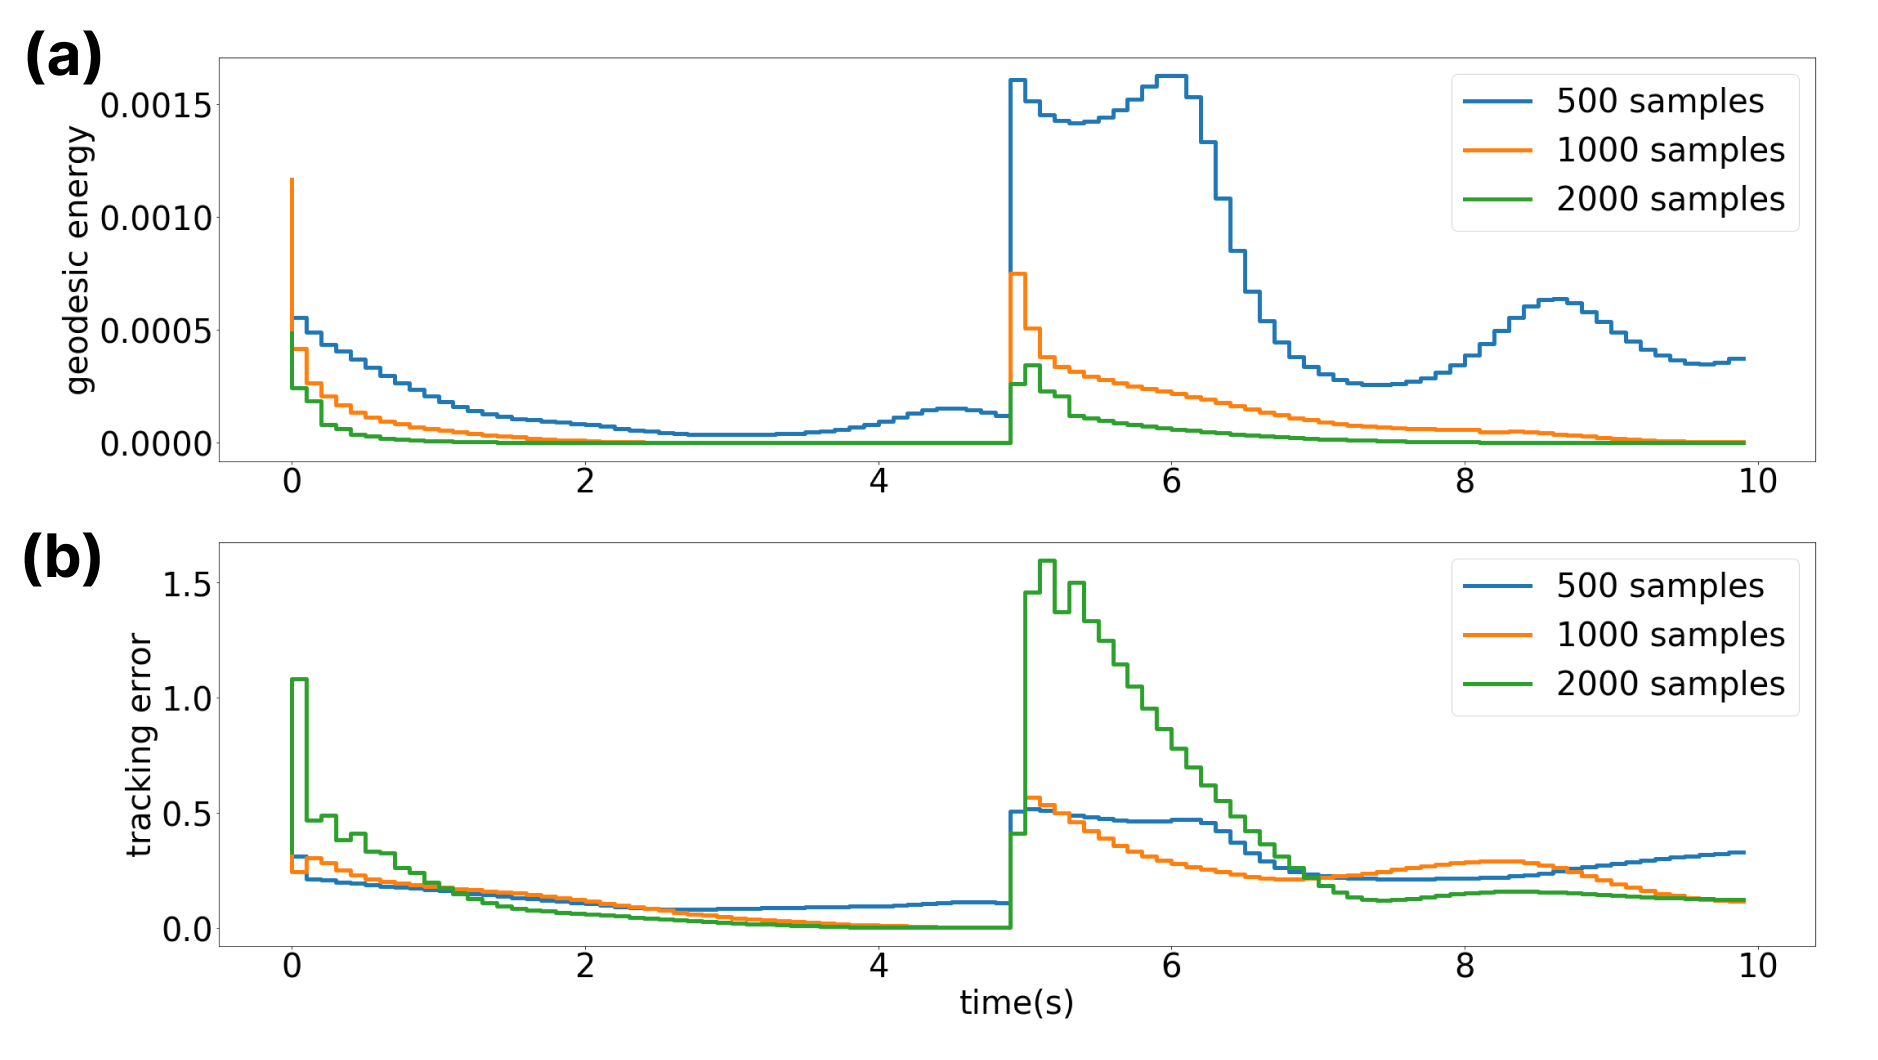
\includegraphics[width = 0.47 \textwidth]
	{figures/comparison_num_samples.png}
    \caption{Comparison of performance of controllers synthesized with varying numbers of samples. Parameters listed in table (\ref{table:comparison_num_sample_params}); (\textbf{a}) geodesic energy $E(\bar{\gamma})$, (\ref{eq:geodesic_length_energy}), (\ref{eq:geodesic_opt}); (\textbf{b}) $l_2$-norm tracking error.}
	\label{fig:comparison_num_sample}
\end{figure}

\subsection{Discretization of Geodesic} \label{sec:discretization_geodesic}
In testing, we found that trying to find the geodesic for the planar pushing system with $N>1$ (\ref{eq:geodesic_opt}) consistently failed. This was slightly unexpected as even though there are more decision variables for larger $N$, and while acknowledging that this is a non-convex problem, it was interesting that SNOPT was not able to find even the straight line solution. We were able to get larger $N$s in our implementation of the simpler 2-dimensional CSTR dynamical system from \autocite{weiControlContractionMetric2021}, but did notice that it significantly increased the online computation time.

For future work, we hope to explore warm-starting the larger $N$ geodesic optimization with the solution of the $N=1$ geodesic, and then warm starting subsequent geodesic optimizations with the previous time-step's solution. Given smoothness of the system and the metric, the previous solution should serve as a good inital guess.

\subsection{Effect of Convergence Rates on DCCM Synthesis}
Another peculiar observation of our implementation was that synthesis of the DCCM consistently failed when using $\beta > 0.3$. We would think that it would be strictly easier to satify the slower convergence rate enforced by a larger $\beta$, however this is not what we found. Furthermore, while we were able to synthesize a DCCM with 500 samples for both $\beta = 0.1$ and $\beta = 0.3$, the $\beta = 0.1$ controller was able to stabilize the system while the $\beta = 0.3$ controller was not. This may speak to the brittleness of the controller when using insufficient samples or it may be indicative of some underlying issue that is also contributing the the synthesis of controllers with larger $\beta$ failing. More investigation into this issue is required to fully understand it.

\subsection{Computation Time}
The DCCM synthesis with a monomial basis of degree 4 and 500 samples took approximately 18 minutes, while using a degree 6 basis with the same number of samples took approximately 3 hours and 20 minutes. The synthesis of the DCCM with degree 4 basis and 2000 samples shown in figure \ref{fig:result_2000} took approximately 1 hour.

Online computation of the 1-segment geodesic for a DCCM synthesized with degree 4 basis took 1.54 seconds, while the DCCM synthesized with degree 6 basis took 3.81 seconds.

All experiments were run on a Linux machine with 31.3GB of RAM, an with an Intel Core i7-6700 CPU @ 3.40GHz x 8 processor.

\section{Conclusion and Future Work}
The feasibility of synthesizing and running a DCCM controller on a planar pushing system with smoothed dynamics was demonstrated in this paper. Limitations of this preliminary implementation were also discussed. Unfortunately, in this work we were largely unable to achieve the benefits discussed in section (\ref{sec:introduction}):
\begin{enumerate}
	\item {\bf Certificates of stability and convergence rates}. Two major gaps remain to be overcome in order to certify the stability and performance of a DCCM controller on a real system. The first is that theoretical arguments need to be made about density of samples on which the contraction condition is enforced and a connection drawn to the smoothness of the system in order to bound the error between the closed loop dynamics of the sample-based DCCM, and the smoothed dynamics. Second, the error between the smooth dynamics and exact dynamics also needs to be bounded. Only after mathematically accounting for these two sources of "sim to real" gap will we be able to certify the controller on the real system.
	\item {\bf Trajectory independent controllers}. We were not able to realize this benefit in our implementation due to computational limitations on the number of samples we could add to our synthesis SOS program. This resulted in low coverage of the state space and meant that there was only a narrow basin of attraction around our desired trajectory.
	\item {\bf Convex synthesis of the controller}. While SOS programming was able to synthesize DCCMs that worked, we ran into challenges with the high degree of monomial basis required. Future work should address this issue, possibly by applying more computational power to the system, or exploring other synthesis methods such as learning the contraction metric \autocite{singhLearningStabilizableDynamical2018,chouModelErrorPropagation2021}
	\item {\bf Faster online computation of the control law}. In this paper we used a basic implementation of the geodesic calculation. We avoided working with the symbolic inversion of the $W$ matrix in (\ref{eq:geodesic_opt}) but that made the burden of finding the inverse to the optimizer. In future work, more advanced methods should be explored, such as the warm starting schemes described in section (\ref{sec:discretization_geodesic}) or the pseudospectral approach described in \autocite{leungNonlinearStabilizationControl2017}.
\end{enumerate}

Another interesting direction we are excited to explore is reformulating the problem such that we only care about stabilizing the state of the object to the desired trajectory and do not require the trajectories of the robot to be contracting. Stability and tabilization of submanifolds were briefly discussed in \autocite{manchesterControlContractionMetrics2017}, but more work need to be done to translate it to the discrete-time case. This formulation may be more true to our goals of manipulating the object and reduce the dimensionality of the problem which might make both offline and online calculations easier.

While more work needs to be done to realize the full benefits of applying the control contraction metric framework to the problem of control through contact, we are hopeful that this paper serves as a good first step on that path.

\printbibliography

\end{document}
